

%----------------------------------------------------------------------------------------
%	PACKAGES AND OTHER DOCUMENT CONFIGURATIONS
%----------------------------------------------------------------------------------------

\documentclass[12pt]{article}
 
\usepackage{polski}
\usepackage[polish]{babel}
\usepackage[utf8]{inputenc}
\usepackage{datetime}
\usepackage{graphicx}
\usepackage{tikz} 
\usepackage{amsmath}
\usepackage{epstopdf}
\usepackage{array,booktabs}
\usepackage{float}
%\usepackage[colorlinks=true]{hyperref}
%\usepackage[all]{hypcap}
%\usepackage{showframe}
\usepackage{geometry}
 \geometry{
 a4paper, 
 left=30mm,
 right=30mm,
 top=30mm,
 bottom=30mm,
 }
 
\newdate{create_date}{29}{04}{2014}

%----------------------------------------------------------------------------------------

%----------------------------------------------------------------------------------------
% TIKZ PACKAGES
%----------------------------------------------------------------------------------------

\usetikzlibrary{arrows, calc}

%----------------------------------------------------------------------------------------

\begin{document}

\begin{titlepage}

\newcommand{\HRule}{\rule{\linewidth}{0.5mm}}
% Defines a new command for the horizontal lines, change thickness here

\center
% Center everything on the page
 
%----------------------------------------------------------------------------------------
%	LOGO SECTION
%----------------------------------------------------------------------------------------


\includegraphics[width=6cm]{../res/img/logo.png}\\[1cm]
% Include a department/university logo - this will require the graphicx package
 
%----------------------------------------------------------------------------------------
 
%----------------------------------------------------------------------------------------
%	HEADING SECTIONS
%----------------------------------------------------------------------------------------

\textsc{\LARGE Akademia Górniczo-Hutnicza \\[0.2cm]
im. Stanisława Staszica w Krakowie}\\[1.5cm]
% Name of your university/college

\textsc{\Large Podstawy Automatyki}\\[0.5cm]
% Major heading such as course name

%----------------------------------------------------------------------------------------
%	TITLE SECTION
%----------------------------------------------------------------------------------------

\HRule \\[0.5cm]
{ \huge \bfseries Dyskretne układy regulacji \\[0.3cm] oraz \\[0.5cm] Analiza
serwomechanizmu \\[0.2cm] przekaźnikowego z wykorzystaniem płaszczyzny
fazowej}\\[0.3cm]
% Title of your document
\HRule \\[1.5cm]
 
%----------------------------------------------------------------------------------------
%	AUTHOR SECTION
%----------------------------------------------------------------------------------------

% \begin{minipage}{0.4\textwidth}
% \begin{flushleft} \large
% \emph{Author:}\\
% Konrad \textsc{Adasiewcz} % Your name
% \end{flushleft}
% \end{minipage}
% ~
% \begin{minipage}{0.4\textwidth}
% \begin{flushright} \large
% \emph{Supervisor:} \\
% dr inż. Paweł \textsc{Rotter} % Supervisor's Name
% \end{flushright}
% \end{minipage}\\[4cm]

% If you don't want a supervisor, uncomment the two lines below and remove the section above
\flushright
\Large \emph{Autorzy:}\\
Konrad \textsc{Adasiewcz}\\[0.1cm] % Your name
Michał \textsc{Maciejewski}\\[3cm] % Your name

%----------------------------------------------------------------------------------------
%	DATE SECTION
%----------------------------------------------------------------------------------------
Data wykonania ćwiczenia: \\
{\large \displaydate{exercise_date}}\\[1cm]


\vfill % Fill the rest of the page with whitespace

\end{titlepage}

\section{Wstęp}

\subsection{Cel ćwiczenia}
Celem ćwiczenia jest wykonanie modelu urządzenia hamującego lądujące na
lotniskowcach samoloty.

\subsection{Zadanie wprowadzające 1}

Zadaniem wprowadzającym jest wykonanie liniowego modelu prostego układu
masa-sprężyna. Poniżej zamieszczam jego schemat:

\begin{figure}[!htb] 
	\begin{center}
		\pgfmathsetmacro{\bloczekr}{50}

\def\bloczek at (#1,#2){
	\draw 	(#1,#2) circle (\bloczekr/3 pt)
			(#1,#2) circle (\bloczekr pt)
}

\def\masa at (#1,#2){
	\draw 	(#1-2.5*\bloczekr pt,#2-1.5*\bloczekr pt)
			rectangle +(5*\bloczekr pt,3*\bloczekr pt)
}

\def\sprezyna at (#1,#2){
	\draw	(#1,#2) --
			++(180:50pt)--
			++(120:50pt) --
			++(-120:100pt)--
			++(120:100pt) --
			++(-120:100pt)--
			++(120:100pt) --
			++(-120:100pt) --
			++(120:50pt) --
			++(180:50pt);
}

\def\gndhr at (#1,#2){
	\draw	(#1,#2)
			++(0,-2.5*\bloczekr pt) --
			++(0,5*\bloczekr pt);
	\foreach \y in {0,1,2,3,4}{
		\draw 	(#1,#2)
				++(0,-2.5*\bloczekr pt+\y*\bloczekr pt) --
				+(135:50pt);
	}
}

\def\gndhl at (#1,#2){
	\draw	(#1,#2)
			++(0,-2.5*\bloczekr pt) --
			++(0,5*\bloczekr pt);
	\foreach \y in {0,1,2,3,4}{
		\draw 	(#1,#2)
				++(0,-2.5*\bloczekr pt+\y*\bloczekr pt) --
				+(45:50pt);
	}
}

\def\gndvd at (#1,#2){
	\draw	(#1,#2)
			++(-2.5*\bloczekr pt,0) --
			++(5*\bloczekr pt,0);
	\foreach \y in {0,1,2,3,4}{
		\draw 	(#1,#2)
				++(-2.5*\bloczekr pt+\y*\bloczekr pt,0) --
				+(45:50pt);
	}
}

\def\gndvu at (#1,#2){
	\draw	(#1,#2)
			++(-2.5*\bloczekr pt,0) --
			++(5*\bloczekr pt,0);
	\foreach \y in {0,1,2,3,4}{
		\draw 	(#1,#2)
				++(-2.5*\bloczekr pt+\y*\bloczekr pt,0) --
				+(-45:50pt);
	}
}

\begin{tikzpicture}[scale=0.15]

\draw[very thick,-latex]
	(-1300pt,300pt) -- node[below]{$$}
	(-800pt,300pt);

\masa at (0,0); %m1
\draw	(0,0)
		++(0,130pt) node{$m_1$};
\coordinate (mz) at (-2.5*\bloczekr pt, 0);

\draw 	(mz) --
		++(-300pt,0);
\sprezyna at (-2.5*\bloczekr pt - 300pt, 0);

\draw	(-2.5*\bloczekr pt - 300pt, 0)
		++(-200pt,-120pt) node{$k_1$};

\draw 	(-2.5*\bloczekr pt - 700pt, 0) --
		(-2.5*\bloczekr pt - 1000pt, 0);

\gndhr at (-2.5*\bloczekr pt - 1000pt, 0);


\end{tikzpicture}
		\caption{Schemat kinematyczny układu masa-sprężyna}
		\label{rys:wpr_spr_sch} 
	\end{center}
\end{figure}

Równanie różniczkowe opisujące ruch masy $m_1$ ma postać:

\begin{equation}
	m_1\ddot{x}=-k_1x
\end{equation}

Stosując standardowe podstawienie $x_1 = x$, $\dot{x_1} = \dot{x}$ $x_2 =
\dot{x_1} = \dot{x}$, $\dot{x_2} = \ddot{x}$ otrzymujemy układ dwóch równań
różniczkowych rzędu I:

\begin{equation}
	\dot{X} =
	\begin{bmatrix}
		0 & 1 \\
		-\frac{k_1}{m_1} & 0
	\end{bmatrix}
	X, \hspace{1cm}
	X =
	\begin{bmatrix}
		x_1 \\
		x_2
	\end{bmatrix}
\end{equation}

Macierze równania stanu dla rozpatrywanego układu mają postać:

\begin{equation*}
	\begin{array}{r l}
		A = &
		\begin{bmatrix}
			0 & 1 \\
			-\frac{k_1}{m_1} & 0
		\end{bmatrix} \\[0.5cm]
		B = &
		\begin{bmatrix}
			0 \\
			0
		\end{bmatrix} \\[0.5cm]
		C = &
		\begin{bmatrix}
			1 & 0 \\
		\end{bmatrix} \\[0.5cm]
		D = & 0 \\
	\end{array}
\end{equation*}

Model został zaimplementowany na cztery sposoby przedstawione niżej.
Współczynnik sprężystości sprężyny $k_1 = 6[\frac{kN}{m}]$, masa
$m_1 = 14000[kg]$. warunki początkowe: $x = 0[m]$, $\dot{x} = 70[\frac{m}{s}]$.

\newpage

\begin{figure}[!htb]
	\begin{center}
		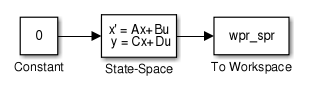
\includegraphics[width=5cm]{../res/img/wpr_sprA_mdl.png}
	\end{center}
	\caption{Schemat modelu zrealizowany z użyciem bloku \textit{State-Space}}
	\label{rys:sch_wpr_mdlA}
\end{figure}

\begin{figure}[!htb]
	\begin{center}
		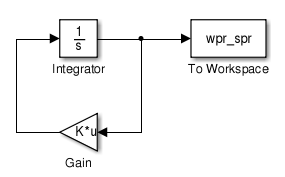
\includegraphics[width=5cm]{../res/img/wpr_sprB_mdl.png}
	\end{center}
	\caption{Schemat modelu zrealizowany z użyciem integratora, i macierzą w pętli
	sprzężenia zwrotnego}
	\label{rys:sch_wpr_mdlB}
\end{figure}

\begin{figure}[!htb]
	\begin{center}
		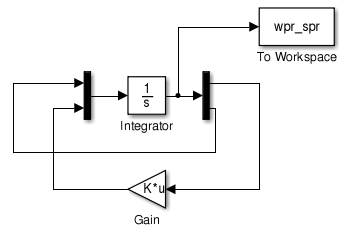
\includegraphics[width=6cm]{../res/img/wpr_sprC_mdl.png}
	\end{center}
	\caption{Schemat modelu zrealizowany z użyciem integratora, oraz
	demultipleksacji i multipleksacji wektora stanu w pętli sprzężenia zwrotnego}
	\label{rys:sch_wpr_mdlC}
\end{figure}

\begin{figure}[!htb]
	\begin{center}
		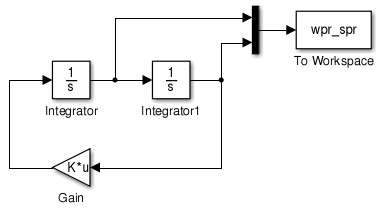
\includegraphics[width=6cm]{../res/img/wpr_sprD_mdl.png}
	\end{center}
	\caption{Schemat modelu zrealizowany z użyciem integratora, oraz
	demultipleksacji i multipleksacji wektora stanu w pętli sprzężenia zwrotnego}
	\label{rys:sch_wpr_mdlD}
\end{figure}

\newpage

Odpowiedzi wszystkich powyższych modeli są identyczne i prezentują się
następująco:

\begin{figure}[!htb]
	\begin{center}
		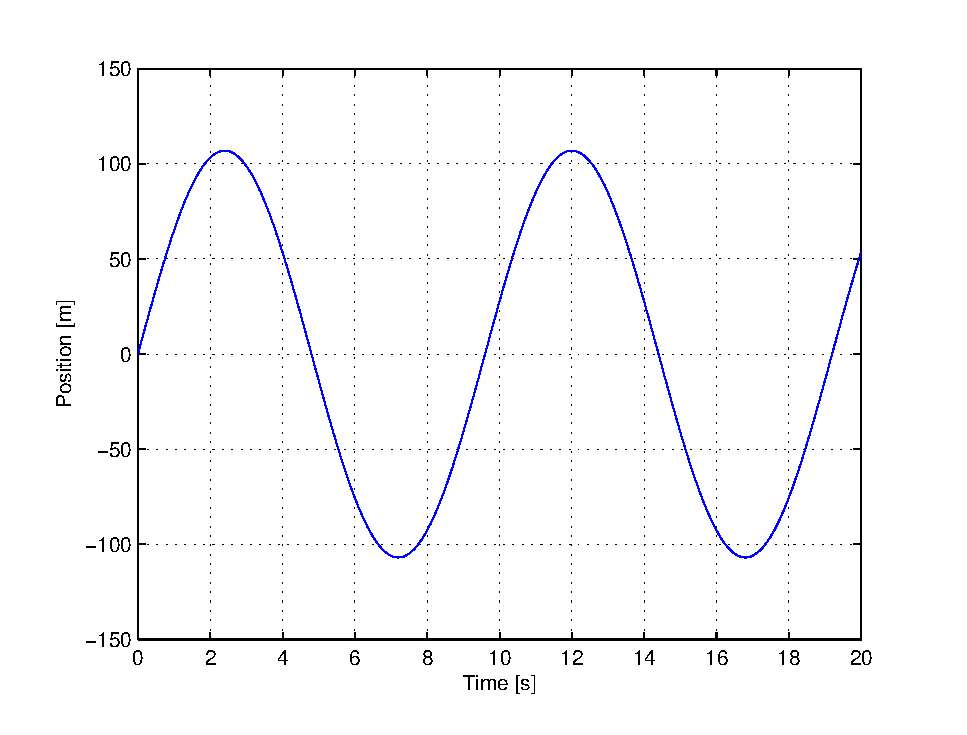
\includegraphics[width=14cm]{../res/img/wpr_spr.eps}
	\end{center} 
	\caption{Przebieg położenia masy $m_1$ w funkcji czasu dla założonych
	parametrów modelu}
	\label{rys:wpr_spr}
\end{figure}

\newpage

\subsection{Zadanie wprowadzające 2 - modelowanie nieliniowości}

Praca poniższego układu mechanicznego jest opisana nieliniowymi równaniami
różniczkowymi.

\begin{figure}[!htb]
	\begin{center}
		\pgfmathsetmacro{\bloczekr}{50}

\def\bloczek at (#1,#2){
	\draw 	(#1,#2) circle (\bloczekr/3 pt)
			(#1,#2) circle (\bloczekr pt)
}

\def\masa at (#1,#2){
	\draw 	(#1-2.5*\bloczekr pt,#2-1.5*\bloczekr pt)
			rectangle +(5*\bloczekr pt,3*\bloczekr pt)
}

\def\sprezyna at (#1,#2){
	\draw	(#1,#2) --
			++(180:50pt)--
			++(120:50pt) --
			++(-120:100pt)--
			++(120:100pt) --
			++(-120:100pt)--
			++(120:100pt) --
			++(-120:100pt) --
			++(120:50pt) --
			++(180:50pt);
}

\def\gndhr at (#1,#2){
	\draw	(#1,#2)
			++(0,-2.5*\bloczekr pt) --
			++(0,5*\bloczekr pt);
	\foreach \y in {0,1,2,3,4}{
		\draw 	(#1,#2)
				++(0,-2.5*\bloczekr pt+\y*\bloczekr pt) --
				+(135:50pt);
	}
}

\def\gndhl at (#1,#2){
	\draw	(#1,#2)
			++(0,-2.5*\bloczekr pt) --
			++(0,5*\bloczekr pt);
	\foreach \y in {0,1,2,3,4}{
		\draw 	(#1,#2)
				++(0,-2.5*\bloczekr pt+\y*\bloczekr pt) --
				+(45:50pt);
	}
}

\def\gndvd at (#1,#2){
	\draw	(#1,#2)
			++(-2.5*\bloczekr pt,0) --
			++(5*\bloczekr pt,0);
	\foreach \y in {0,1,2,3,4}{
		\draw 	(#1,#2)
				++(-2.5*\bloczekr pt+\y*\bloczekr pt,0) --
				+(45:50pt);
	}
}

\def\gndvu at (#1,#2){
	\draw	(#1,#2)
			++(-2.5*\bloczekr pt,0) --
			++(5*\bloczekr pt,0);
	\foreach \y in {0,1,2,3,4}{
		\draw 	(#1,#2)
				++(-2.5*\bloczekr pt+\y*\bloczekr pt,0) --
				+(-45:50pt);
	}
}

\begin{tikzpicture}[scale=0.12]

\draw[very thick,-latex]
	(-1800pt,0) -- node[below]{$$}
	(-800pt,0);

\masa at (0,0); %m1
\draw	(0,0)
		++(0,130pt) node{$m_1$};
\coordinate (mz) at (-2.5*\bloczekr pt, 0);

\draw	(mz) -- node[below]{$x$}
		(-10*\bloczekr pt,0) -- node[left]{$h$}
		(-10*\bloczekr pt, 10*\bloczekr pt);
\draw	(-10*\bloczekr pt,0)
		++(0,10*\bloczekr*1.17 pt)
		++(0,-300pt)
		arc (-90:-57:300pt)
		+(-100pt,50pt) node{$\theta$};

\bloczek at (-10*\bloczekr pt, 10*\bloczekr pt); %b1
\draw 	(mz) -- 
		($(-10*\bloczekr pt, 10*\bloczekr pt) + 
		({atan(0.75)}:\bloczekr pt)$);
\draw	($(-10*\bloczekr pt, 10*\bloczekr pt) + 
		(90:\bloczekr pt)$) --
		(-16*\bloczekr pt, 11*\bloczekr pt);
\sprezyna at (-16*\bloczekr pt, 11*\bloczekr pt); %k1
\draw	(-16*\bloczekr pt, 11*\bloczekr pt)
		++(-200pt,-120pt) node{$k_1$};
\draw 	($(-16*\bloczekr pt, 11*\bloczekr pt) +
		(-400pt,0)$) --
		($(-30*\bloczekr pt, 12*\bloczekr pt) +
		(-90:\bloczekr pt)$);
\gndhr at (-16*\bloczekr pt - 700pt, 11*\bloczekr pt);

\begin{scope}[yscale=-1]
	\bloczek at (-10*\bloczekr pt, 10*\bloczekr pt); %b1
	\draw 	(mz) -- 
			($(-10*\bloczekr pt, 10*\bloczekr pt) + 
			({atan(0.75)}:\bloczekr pt)$);
	\draw	($(-10*\bloczekr pt, 10*\bloczekr pt) + 
			(90:\bloczekr pt)$) --
			(-16*\bloczekr pt, 11*\bloczekr pt);
	\sprezyna at (-16*\bloczekr pt, 11*\bloczekr pt); %k1
	\draw	(-16*\bloczekr pt, 11*\bloczekr pt)
			++(-200pt,-120pt) node{$k_1$};
	\draw 	($(-16*\bloczekr pt, 11*\bloczekr pt) +
			(-400pt,0)$) --
			($(-30*\bloczekr pt, 12*\bloczekr pt) +
			(-90:\bloczekr pt)$);
	\gndhr at (-16*\bloczekr pt - 700pt, 11*\bloczekr pt);
\end{scope}


\end{tikzpicture}
		\caption{Schemat kinematyczny nieliniowego układu sprężyn}
		\label{rys:wpr_spr_nl_sch}
	\end{center}
\end{figure}

Ich postać jest następująca:

\begin{equation}
	\begin{cases}
		\dot{x_1} = & x_2 \\
		\dot{x_2} = & -\frac{k_1}{m_1}g(x_1)
	\end{cases}
\end{equation}

gdzie:

\begin{equation}
	g(x) = \left(1-\frac{h}{\sqrt{x^2+h^2}}\right)x \\[0.5cm]
\end{equation}

Model został wykonany w zmodyfikowany sposób z rysunku \ref{rys:sch_wpr_mdlC}

\begin{figure}[!htb]
	\begin{center}
		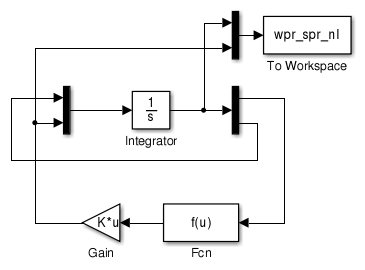
\includegraphics[width=7cm]{../res/img/wpr_spr_nl_mdl.png}
	\end{center} 
	\caption{Schemat modelu zrealizowany z użyciem integratora, oraz
	demultipleksacji i multipleksacji wektora stanu w pętli sprzężenia zwrotnego,
	z uwzględnieniem nieliniowości modelu}
	\label{rys:wpr_spr_nl_mdl}
\end{figure}

Praca układu dla parametrów $k_1 = 200[\frac{kN}{m}]$, masa
$m_1 = 14000[kg]$, $h = 40[m]$. warunki początkowe: $x = 0[m]$, $\dot{x} =
70[\frac{m}{s}]$ jest przedstawiona na poniższym wykresie:

\begin{figure}[!htb]
	\begin{center}
		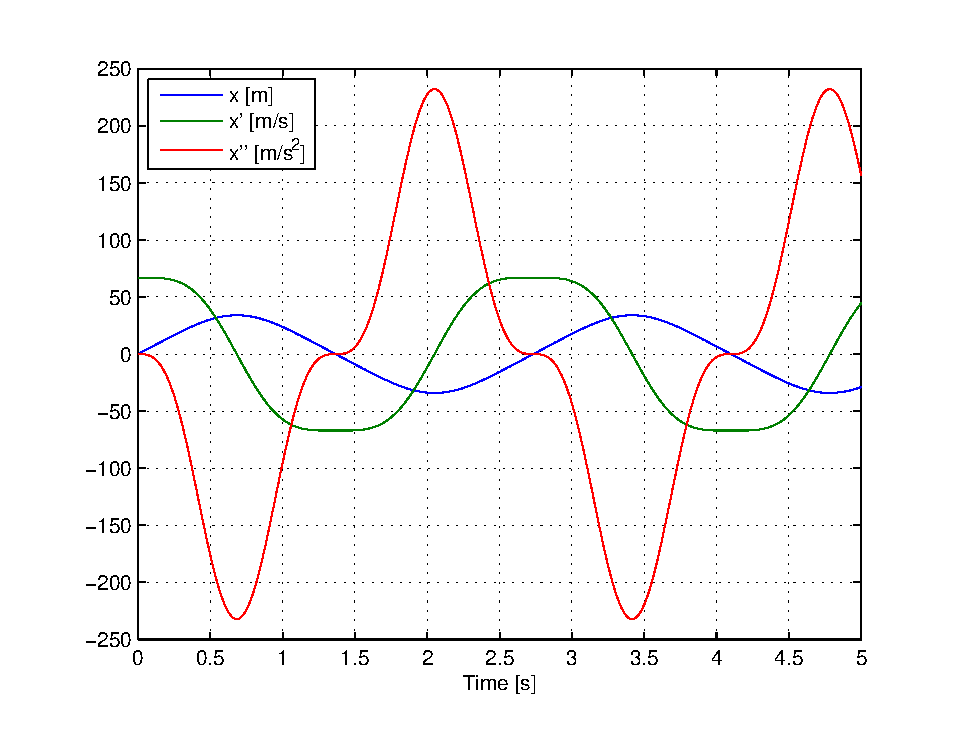
\includegraphics[width=14cm]{../res/img/wpr_spr_nl.eps}
	\end{center} 
	\caption{Przebieg położenia, prędkości oraz
	przyspieszenia masy $m_1$ w funkcji czasu dla założonych parametrów modelu} 
	\label{rys:wpr_spr_nl} 
\end{figure}

\newpage

\subsection{Zadanie wprowadzające 3 - model urządzenia hamującego bez tłumików
wodnych}

Prostsza wersja docelowego urządzenia różni się od układu z poprzedniego punktu
obecnością dodatkowej masy i sprężyny na stronę.

\begin{figure}[!htb]
	\begin{center}
		\pgfmathsetmacro{\bloczekr}{50}

\def\bloczek at (#1,#2){
	\draw 	(#1,#2) circle (\bloczekr/3 pt)
			(#1,#2) circle (\bloczekr pt)
}

\def\masa at (#1,#2){
	\draw 	(#1-2.5*\bloczekr pt,#2-1.5*\bloczekr pt)
			rectangle +(5*\bloczekr pt,3*\bloczekr pt)
}

\def\sprezyna at (#1,#2){
	\draw	(#1,#2) --
			++(180:50pt)--
			++(120:50pt) --
			++(-120:100pt)--
			++(120:100pt) --
			++(-120:100pt)--
			++(120:100pt) --
			++(-120:100pt) --
			++(120:50pt) --
			++(180:50pt);
}

\def\gndhr at (#1,#2){
	\draw	(#1,#2)
			++(0,-2.5*\bloczekr pt) --
			++(0,5*\bloczekr pt);
	\foreach \y in {0,1,2,3,4}{
		\draw 	(#1,#2)
				++(0,-2.5*\bloczekr pt+\y*\bloczekr pt) --
				+(135:50pt);
	}
}

\def\gndhl at (#1,#2){
	\draw	(#1,#2)
			++(0,-2.5*\bloczekr pt) --
			++(0,5*\bloczekr pt);
	\foreach \y in {0,1,2,3,4}{
		\draw 	(#1,#2)
				++(0,-2.5*\bloczekr pt+\y*\bloczekr pt) --
				+(45:50pt);
	}
}

\def\gndvd at (#1,#2){
	\draw	(#1,#2)
			++(-2.5*\bloczekr pt,0) --
			++(5*\bloczekr pt,0);
	\foreach \y in {0,1,2,3,4}{
		\draw 	(#1,#2)
				++(-2.5*\bloczekr pt+\y*\bloczekr pt,0) --
				+(45:50pt);
	}
}

\def\gndvu at (#1,#2){
	\draw	(#1,#2)
			++(-2.5*\bloczekr pt,0) --
			++(5*\bloczekr pt,0);
	\foreach \y in {0,1,2,3,4}{
		\draw 	(#1,#2)
				++(-2.5*\bloczekr pt+\y*\bloczekr pt,0) --
				+(-45:50pt);
	}
}

\begin{tikzpicture}[scale=0.13]

\draw[very thick,-latex]
	(-2400pt,0) -- node[below]{$$}
	(-1400pt,0);

\masa at (0,0); %m1
\draw	(0,0)
		++(0,130pt) node{$m_1$};
\coordinate (mz) at (-2.5*\bloczekr pt, 0);

\draw	(mz) -- node[below]{$x$}
		(-10*\bloczekr pt,0) -- node[left]{$h$}
		(-10*\bloczekr pt, 10*\bloczekr pt);
\draw	(-10*\bloczekr pt,0)
		++(0,10*\bloczekr*1.17 pt)
		++(0,-300pt)
		arc (-90:-57:300pt)
		+(-100pt,50pt) node{$\theta$};

\bloczek at (-10*\bloczekr pt, 10*\bloczekr pt); %b1
\draw 	(mz) -- 
		($(-10*\bloczekr pt, 10*\bloczekr pt) + 
		({atan(0.75)}:\bloczekr pt)$);
\draw	($(-10*\bloczekr pt, 10*\bloczekr pt) + 
		(90:\bloczekr pt)$) --
		(-16*\bloczekr pt, 11*\bloczekr pt);
\sprezyna at (-16*\bloczekr pt, 11*\bloczekr pt); %k1
\draw	(-16*\bloczekr pt, 11*\bloczekr pt)
		++(-200pt,-120pt) node{$k_1$};
\draw 	($(-16*\bloczekr pt, 11*\bloczekr pt) +
		(-400pt,0)$) --
		($(-30*\bloczekr pt, 12*\bloczekr pt) +
		(-90:\bloczekr pt)$);
\bloczek at (-30*\bloczekr pt, 12*\bloczekr pt); %b3
\masa at (-30*\bloczekr pt, 12*\bloczekr pt); %m2
\draw	(-30*\bloczekr pt, 12*\bloczekr pt)
		++(0,130pt) node{$m_2$};
\draw 	($(-30*\bloczekr pt, 12*\bloczekr pt) +
		(90:\bloczekr pt)$) --
		($(-10*\bloczekr pt, 14*\bloczekr pt) +
		(-90:\bloczekr pt)$);
\bloczek at (-10*\bloczekr pt, 14*\bloczekr pt); %b2
\draw 	(-30*\bloczekr pt, 12*\bloczekr pt)
		++(-2.5*\bloczekr pt, 0) --
		++(-200pt,0);
\draw	(-10*\bloczekr pt, 14*\bloczekr pt)
		++(\bloczekr pt, 0) --
		++(0,200pt);
\gndvd at (-9*\bloczekr pt, 14*\bloczekr pt + 200pt);
\sprezyna at (-30*\bloczekr pt -2.5*\bloczekr pt-200pt, 12*\bloczekr pt); %k2
\draw	(-30*\bloczekr pt -2.5*\bloczekr pt-200pt, 12*\bloczekr pt)
		++(-200pt,-120pt) node{$k_2$};
\draw	(-30*\bloczekr pt -2.5*\bloczekr pt-600pt, 12*\bloczekr pt) --
		++(-200pt,0);
\gndhr at (-30*\bloczekr pt -2.5*\bloczekr pt-800pt, 12*\bloczekr pt);

\begin{scope}[yscale=-1]
	\bloczek at (-10*\bloczekr pt, 10*\bloczekr pt); %b1
	\draw 	(mz) -- 
			($(-10*\bloczekr pt, 10*\bloczekr pt) + 
			({atan(0.75)}:\bloczekr pt)$);
	\draw	($(-10*\bloczekr pt, 10*\bloczekr pt) + 
			(90:\bloczekr pt)$) --
			(-16*\bloczekr pt, 11*\bloczekr pt);
	\sprezyna at (-16*\bloczekr pt, 11*\bloczekr pt); %k1
	\draw	(-16*\bloczekr pt, 11*\bloczekr pt)
			++(-200pt,-120pt) node{$k_1$};
	\draw 	($(-16*\bloczekr pt, 11*\bloczekr pt) +
			(-400pt,0)$) --
			($(-30*\bloczekr pt, 12*\bloczekr pt) +
			(-90:\bloczekr pt)$);
	\bloczek at (-30*\bloczekr pt, 12*\bloczekr pt); %b3
	\masa at (-30*\bloczekr pt, 12*\bloczekr pt); %m2
	\draw	(-30*\bloczekr pt, 12*\bloczekr pt)
			++(0,130pt) node{$m_2$};
	\draw 	($(-30*\bloczekr pt, 12*\bloczekr pt) +
			(90:\bloczekr pt)$) --
			($(-10*\bloczekr pt, 14*\bloczekr pt) +
			(-90:\bloczekr pt)$);
	\bloczek at (-10*\bloczekr pt, 14*\bloczekr pt); %b2
	\draw 	(-30*\bloczekr pt, 12*\bloczekr pt)
			++(-2.5*\bloczekr pt, 0) --
			++(-200pt,0);
	\draw	(-10*\bloczekr pt, 14*\bloczekr pt)
			++(\bloczekr pt, 0) --
			++(0,200pt);
	\gndvd at (-9*\bloczekr pt, 14*\bloczekr pt + 200pt);
	\sprezyna at (-30*\bloczekr pt -2.5*\bloczekr pt-200pt, 12*\bloczekr pt); %k2
	\draw	(-30*\bloczekr pt -2.5*\bloczekr pt-200pt, 12*\bloczekr pt)
			++(-200pt,-120pt) node{$k_2$};
	\draw	(-30*\bloczekr pt -2.5*\bloczekr pt-600pt, 12*\bloczekr pt) --
			++(-200pt,0);
	\gndhr at (-30*\bloczekr pt -2.5*\bloczekr pt-800pt, 12*\bloczekr pt);
\end{scope}

\end{tikzpicture}
		\caption{Schemat kinematyczny urządzenia hamującego bez tłumików}
		\label{rys:wpr_hamsam_sch}
	\end{center}
\end{figure}

Wymusza to konieczność dodania zmiennej $y_2$ odpowiadającej za położenie masy
$m_2$. Sprowadza to równania różniczkowe opisujące model do postaci:

\begin{equation}
	\begin{cases}
		\ddot{x} = \frac{1}{m_1}(4k_1y_2-2k_1y_1)\sin\theta \\
		\ddot{y_2} = \frac{1}{m_2}\left[-(4k_1+k_2)y_2+2k_1y_1\right]
	\end{cases}
\end{equation}

\vspace{0.5cm}

gdzie $y_1 = \sqrt{x^2+h^2} - h$

\vspace{0.5cm}

Parametry modelu: $k_1 = 55[\frac{kN}{m}]$, $k_2 = 300[\frac{kN}{m}]$, masa
$m_1 = 14000[kg]$, $m_2 = 500[kg]$, $h = 40[m]$. warunki początkowe: $x =
0[m]$, $\dot{x} = 70[\frac{m}{s}]$.
\newpage

\begin{figure}[!htb]
	\begin{center}
		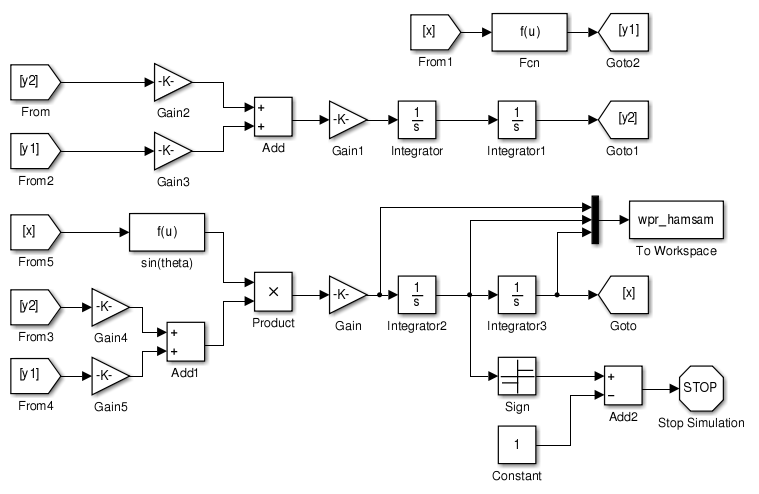
\includegraphics[width=12cm]{../res/img/wpr_hamsam_mdl.png}
	\end{center} 
	\caption{Schemat modelu zrealizowany z użyciem integratorów 1D}
	\label{rys:wpr_hamsam_mdl}
\end{figure}

\vspace{0.5cm}

Tak skonstruowany model spełnia swoje zadanie, jednak przeciążenia działające na
pilota w czasie lądowania są na tyle duże iż z dużym prawdopodobieństwem
straci on przytomność. Poniżej stosowne przebiegi położenia, prędkości oraz
przyspieszenia samolotu.

\begin{figure}[!htb]
	\begin{center}
		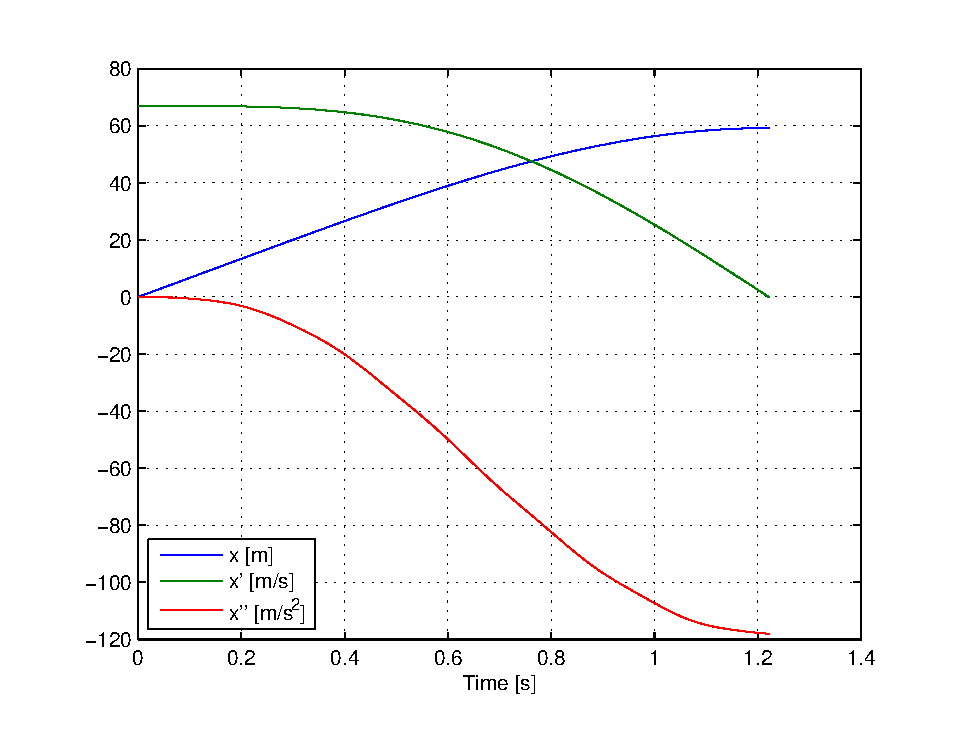
\includegraphics[width=12cm]{../res/img/wpr_hamsam.eps}
	\end{center} 
	\caption{Przebieg położenia, prędkości oraz
	przyspieszenia masy $m_1$ w funkcji czasu dla założonych parametrów modelu} 
	\label{rys:wpr_hamsam} 
\end{figure}

\newpage 

\section{Model właściwego urządzenia}

W stosunku do poprzedniego modelu w równaniach opisujących dynamikę układu
pojawia się kolejna zmienna stanu $y_3$ opisująca położenie tłoka tłumika
wodnego.

\begin{figure}[!htb]
	\begin{center}
		\pgfmathsetmacro{\bloczekr}{50}

\def\bloczek at (#1,#2){
	\draw 	(#1,#2) circle (\bloczekr/3 pt)
			(#1,#2) circle (\bloczekr pt)
}

\def\masa at (#1,#2){
	\draw 	(#1-2.5*\bloczekr pt,#2-1.5*\bloczekr pt)
			rectangle +(5*\bloczekr pt,3*\bloczekr pt)
}

\def\sprezyna at (#1,#2){
	\draw	(#1,#2) --
			++(180:50pt)--
			++(120:50pt) --
			++(-120:100pt)--
			++(120:100pt) --
			++(-120:100pt)--
			++(120:100pt) --
			++(-120:100pt) --
			++(120:50pt) --
			++(180:50pt);
}

\def\gndhr at (#1,#2){
	\draw	(#1,#2)
			++(0,-2.5*\bloczekr pt) --
			++(0,5*\bloczekr pt);
	\foreach \y in {0,1,2,3,4}{
		\draw 	(#1,#2)
				++(0,-2.5*\bloczekr pt+\y*\bloczekr pt) --
				+(135:50pt);
	}
}

\def\gndhl at (#1,#2){
	\draw	(#1,#2)
			++(0,-2.5*\bloczekr pt) --
			++(0,5*\bloczekr pt);
	\foreach \y in {0,1,2,3,4}{
		\draw 	(#1,#2)
				++(0,-2.5*\bloczekr pt+\y*\bloczekr pt) --
				+(45:50pt);
	}
}

\def\gndvd at (#1,#2){
	\draw	(#1,#2)
			++(-2.5*\bloczekr pt,0) --
			++(5*\bloczekr pt,0);
	\foreach \y in {0,1,2,3,4}{
		\draw 	(#1,#2)
				++(-2.5*\bloczekr pt+\y*\bloczekr pt,0) --
				+(45:50pt);
	}
}

\def\gndvu at (#1,#2){
	\draw	(#1,#2)
			++(-2.5*\bloczekr pt,0) --
			++(5*\bloczekr pt,0);
	\foreach \y in {0,1,2,3,4}{
		\draw 	(#1,#2)
				++(-2.5*\bloczekr pt+\y*\bloczekr pt,0) --
				+(-45:50pt);
	}
}

\def\tlumik at (#1,#2){
	\draw	(#1,#2)
			++(150pt,-50pt) --
			++(-150pt,0) --
			++(0,100pt) -- 
			++(150pt,0);
	\draw[ultra thick]
			(#1,#2)
			++(100pt,-50pt) --
			++(0,100pt);
}

\begin{tikzpicture}[scale=0.13]

\draw[very thick,-latex]
	(-2400pt,0) -- node[below]{$$}
	(-1400pt,0);

\masa at (0,0); %m1
\draw	(0,0)
		++(0,130pt) node{$m_1$};
\coordinate (mz) at (-2.5*\bloczekr pt, 0);

\draw	(mz) -- node[below]{$x$}
		(-10*\bloczekr pt,0) -- node[left]{$h$}
		(-10*\bloczekr pt, 10*\bloczekr pt);
\draw	(-10*\bloczekr pt,0)
		++(0,10*\bloczekr*1.17 pt)
		++(0,-300pt)
		arc (-90:-57:300pt)
		+(-100pt,50pt) node{$\theta$};

\bloczek at (-10*\bloczekr pt, 10*\bloczekr pt); %b1
\draw 	(mz) -- 
		($(-10*\bloczekr pt, 10*\bloczekr pt) + 
		({atan(0.75)}:\bloczekr pt)$);
\draw	($(-10*\bloczekr pt, 10*\bloczekr pt) + 
		(90:\bloczekr pt)$) --
		(-16*\bloczekr pt, 11*\bloczekr pt);
\sprezyna at (-16*\bloczekr pt, 11*\bloczekr pt); %k1
\draw	(-16*\bloczekr pt, 11*\bloczekr pt)
		++(-200pt,-120pt) node{$k_1$};
\draw 	($(-16*\bloczekr pt, 11*\bloczekr pt) +
		(-400pt,0)$) --
		($(-30*\bloczekr pt, 12*\bloczekr pt) +
		(-90:\bloczekr pt)$);
\bloczek at (-30*\bloczekr pt, 12*\bloczekr pt); %b3
\masa at (-30*\bloczekr pt, 12*\bloczekr pt); %m2
\draw	(-30*\bloczekr pt, 12*\bloczekr pt)
		++(0,130pt) node{$m_2$};
\draw 	($(-30*\bloczekr pt, 12*\bloczekr pt) +
		(90:\bloczekr pt)$) --
		($(-10*\bloczekr pt, 14*\bloczekr pt) +
		(-90:\bloczekr pt)$);
\bloczek at (-10*\bloczekr pt, 14*\bloczekr pt); %b2
\draw 	(-30*\bloczekr pt, 12*\bloczekr pt)
		++(-2.5*\bloczekr pt, 0) --
		++(-200pt,0);
\draw	(-10*\bloczekr pt, 14*\bloczekr pt)
		++(\bloczekr pt, 0) --
		++(0,200pt);
\gndvd at (-9*\bloczekr pt, 14*\bloczekr pt + 200pt);
\sprezyna at (-30*\bloczekr pt -2.5*\bloczekr pt-200pt, 12*\bloczekr pt); %k2
\draw	(-30*\bloczekr pt -2.5*\bloczekr pt-200pt, 12*\bloczekr pt)
		++(-200pt,-120pt) node{$k_2$};
\draw	(-30*\bloczekr pt -2.5*\bloczekr pt-600pt, 12*\bloczekr pt) --
		++(-100pt,0);
\gndhr at (-30*\bloczekr pt -2.5*\bloczekr pt-800pt, 12*\bloczekr pt);
\tlumik at (-30*\bloczekr pt -2.5*\bloczekr pt-800pt, 12*\bloczekr pt);
\draw (-30*\bloczekr pt -2.5*\bloczekr pt-800pt, 12*\bloczekr pt)
		node[above right,yshift=10pt]{$m_3$};

\begin{scope}[yscale=-1]
	\bloczek at (-10*\bloczekr pt, 10*\bloczekr pt); %b1
	\draw 	(mz) -- 
			($(-10*\bloczekr pt, 10*\bloczekr pt) + 
			({atan(0.75)}:\bloczekr pt)$);
	\draw	($(-10*\bloczekr pt, 10*\bloczekr pt) + 
			(90:\bloczekr pt)$) --
			(-16*\bloczekr pt, 11*\bloczekr pt);
	\sprezyna at (-16*\bloczekr pt, 11*\bloczekr pt); %k1
	\draw	(-16*\bloczekr pt, 11*\bloczekr pt)
			++(-200pt,-120pt) node{$k_1$};
	\draw 	($(-16*\bloczekr pt, 11*\bloczekr pt) +
			(-400pt,0)$) --
			($(-30*\bloczekr pt, 12*\bloczekr pt) +
			(-90:\bloczekr pt)$);
	\bloczek at (-30*\bloczekr pt, 12*\bloczekr pt); %b3
	\masa at (-30*\bloczekr pt, 12*\bloczekr pt); %m2
	\draw	(-30*\bloczekr pt, 12*\bloczekr pt)
			++(0,130pt) node{$m_2$};
	\draw 	($(-30*\bloczekr pt, 12*\bloczekr pt) +
			(90:\bloczekr pt)$) --
			($(-10*\bloczekr pt, 14*\bloczekr pt) +
			(-90:\bloczekr pt)$);
	\bloczek at (-10*\bloczekr pt, 14*\bloczekr pt); %b2
	\draw 	(-30*\bloczekr pt, 12*\bloczekr pt)
			++(-2.5*\bloczekr pt, 0) --
			++(-200pt,0);
	\draw	(-10*\bloczekr pt, 14*\bloczekr pt)
			++(\bloczekr pt, 0) --
			++(0,200pt);
	\gndvd at (-9*\bloczekr pt, 14*\bloczekr pt + 200pt);
	\sprezyna at (-30*\bloczekr pt -2.5*\bloczekr pt-200pt, 12*\bloczekr pt); %k2
	\draw	(-30*\bloczekr pt -2.5*\bloczekr pt-200pt, 12*\bloczekr pt)
			++(-200pt,-120pt) node{$k_2$};
	\draw	(-30*\bloczekr pt -2.5*\bloczekr pt-600pt, 12*\bloczekr pt) --
			++(-100pt,0);
	\gndhr at (-30*\bloczekr pt -2.5*\bloczekr pt-800pt, 12*\bloczekr pt);
	\tlumik at (-30*\bloczekr pt -2.5*\bloczekr pt-800pt, 12*\bloczekr pt);
	\draw (-30*\bloczekr pt -2.5*\bloczekr pt-800pt, 12*\bloczekr pt)
		node[below right,yshift=-10pt]{$m_3$};
\end{scope}


\end{tikzpicture}
		\caption{Schemat kinematyczny urządzenia hamującego}
		\label{rys:zad_hamsam_sch}
	\end{center}
\end{figure}

Równania różniczkowe mają poniższą postać:

\begin{equation}
	\begin{cases}
		m_1\ddot{x} = -2f_{k1}\sin\theta \\
		m_2\ddot{y_2} = 2f_{k1}-f_{k2} \\
		m_3\ddot{y_3} = f_{k2}-f_{b} \\
	\end{cases}
\end{equation}


Dodatkowo po przebyciu $50[m]$ pilot w samolocie uruchamia hamulce, które
działają z siłą hamującą równą $f_h = 0.7g\cdot m_1[N]$.

\vspace{0.5cm}

Siły $f_{k1}$, $f_{k2}$ oraz $f_b$ są dane zależnościami:

\begin{equation*}
	\begin{array}{r l}
		f_{k1} & = 
		\begin{cases}
			k_1(y_1-2y_2) & y_1 \geq 2y_2 \\
			0 & y_1 < 2y_2
		\end{cases}
\\[0.5cm]
		f_{k2} & = 
		\begin{cases}
			k_2(y_2-y_3) & y_2 \geq y_3 \\
			0 & y_2 < y_3
		\end{cases}
\\[0.5cm]
		f_b & = f(y_3)(\dot{y_3})^2
\\[0.5cm]		
		y_1 & = \sqrt{x^2+h^2} - h
	\end{array}
\end{equation*}

\newpage

oraz $f(y)$ dane jest tabelarycznie:

\begin{table}[ht]
	\centering
	\newcommand\VRule[1][\arrayrulewidth]{\vrule width #1}
	\begin{tabular}{!{\VRule[1.5pt]}c|c!{\VRule[1.5pt]}c|c!{\VRule[1.5pt]}}
		\specialrule{1.5pt}{0pt}{0pt}
		$y$ [$m$] & $f\left(y\right)$ [$\frac{kg}{m}$] & $y$ [$m$] &
		$f\left(y\right)$ [$\frac{kg}{m}$] \\ \specialrule{1.5pt}{0pt}{0pt}
		0 & 833 & 80 & 1070 \\ \hline
		10 & 400 & 90 & 1600 \\ \hline
		20 & 160 & 94 & 2100 \\ \hline
		30 & 320 & 98 & 2800 \\ \hline
		40 & 520 & 102 & 4100 \\ \hline
		50 & 520 & 104 & 5000 \\ \hline
		60 & 660 & 107 & 9000 \\ \hline
		70 & 830 & 120 & 9000 \\ \specialrule{1.5pt}{0pt}{0pt}
	\end{tabular}
	\caption{Stablicowana funkcja $f$ tłumika wodnego}
\end{table} 

\begin{figure}[!htb]
	\begin{center}
		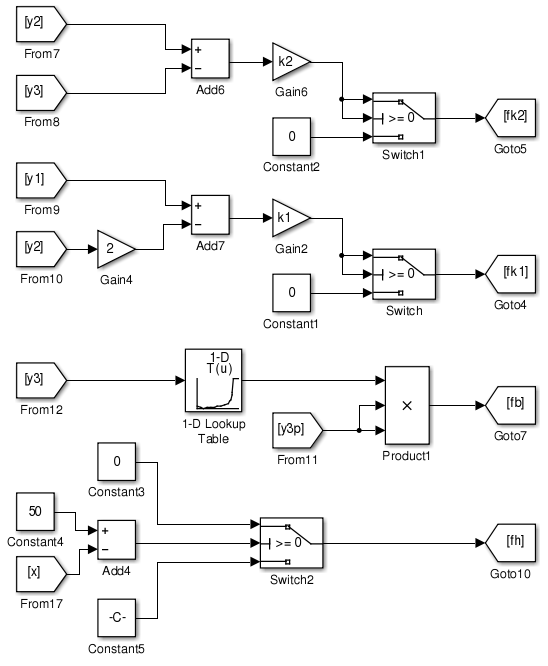
\includegraphics[width=10cm]{../res/img/zad_hamsam_mdl_side.png}
	\end{center} 
	\caption{Boczna część schematu modelu odpowiadająca za obliczanie sił
	działających na poszczególne masy}
	\label{rys:zad_hamsam_mdl_side}
\end{figure}

\newpage

\begin{figure}[!htb]
	\begin{center}
		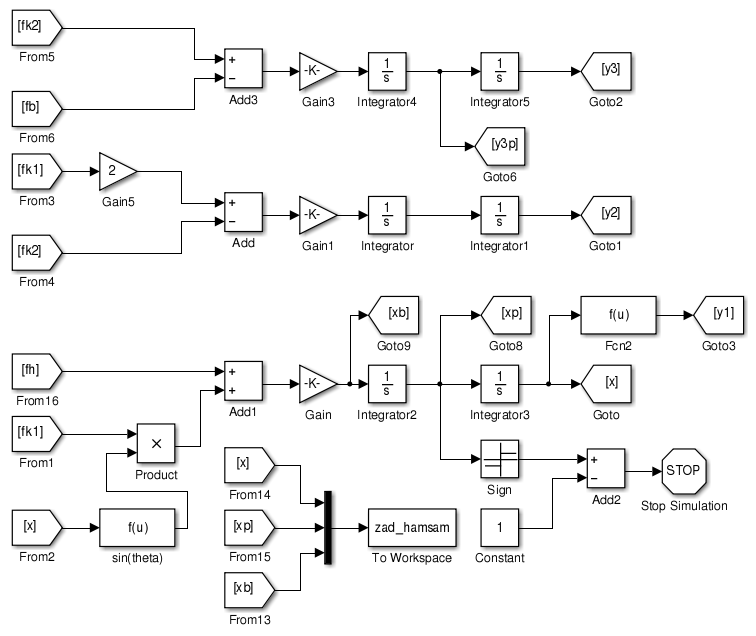
\includegraphics[width=11cm]{../res/img/zad_hamsam_mdl_main.png}
	\end{center} 
	\caption{Główna część schematu modelu rozwiązująca równania
	różniczkowe}
	\label{rys:zad_hamsam_mdl_main}
\end{figure}

Parametry modelu: $k_1 = 54.7[\frac{kN}{m}]$, $k_2 = 303.6[\frac{kN}{m}]$, masa
$m_1 = 14000[kg]$, $m_2 = 450.28[kg]$, $m_3 = 200[kg]$, $h = 42[m]$. warunki
początkowe: $x = 0[m]$, $\dot{x} = 67[\frac{m}{s}]$.

\begin{figure}[!htb]
	\begin{center}
		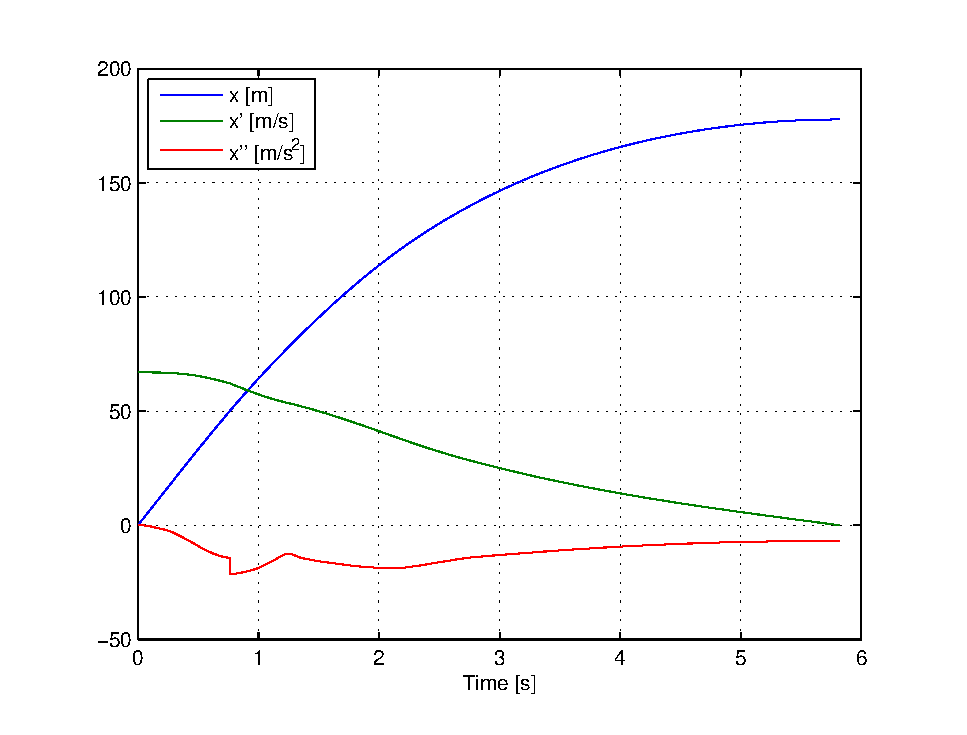
\includegraphics[width=12cm]{../res/img/zad_hamsam.eps}
	\end{center} 
	\caption{Przebieg położenia, prędkości oraz
	przyspieszenia masy $m_1$ w funkcji czasu dla założonych parametrów modelu} 
	\label{rys:zad_hamsam} 
\end{figure}

\clearpage

\section{Wnioski i spostrzeżenia}

Pakiet \textsc{Matlab-Simulink} umożliwia proste modelowanie układów fizycznych
opisanych nieliniowymi równaniami różniczkowymi dzięki dokładnym numerycznym
metodom ich rozwiązywania.

Stworzony model spełnia swoje zadanie - wspomaga zatrzymanie samolotu na krótkim
dystansie przy jednoczesnym ograniczeniu działających nań przyspieszeń.
Oczywiście najbardziej optymistycznym przypadkiem byłaby sytuacja w której
samolot porusza się ze stałym opóźnieniem - wtedy jest ono minimalne a samolot
zatrzymuje się na najkrótszym odcinku drogi.

\end{document}